\section{Virtual PET Images from CT Data Using Deep
Convolutional Networks: Initial Results}

\subsection*{Ссылка}\url{https://arxiv.org/abs/1707.09585}
\subsection*{Введение}
Несмотря на то, что ПЭТ-исследования имеет большое количество положительных 
сторон, у него так же есть и недостатки - радиоактивный компонент опасен 
для беременных и кормящих женщин. Также, ПЭТ - сравнительно новый метод, который все 
еще является дорогостоящим для среднестатистического человека, также возможность получить 
ПЭТ обследование есть не во всех медицинских центрах. Сложность получения ПЭТ-изображений для 
полседующего лечения послужила возникновению идеи поиска альтернативы - менее дорогостоящего, быстрого 
и легко в применении ПЭТ-подобного изображения. В данной работе исследуется 
модуль для созданиявиртуальных ПЭТ-изображений на основе информации из КТ-изображений.
\subsection*{Основная идея}
Фреймворк включает в себя три модуля:
\begin{itemize}
    \item Тренировочный модуль, который также включает в себя предобработку данных;
    \item Тестовый модуль, на вход которому подается КТ-изображение для предсказания 
    ПЭТ-подобного изображения на выходе;
    \item Модуль смешения (blending module), который соединяет выходы FCN и GAN.
\end{itemize}
FCN и GAN участвуют как в тренировке, так и в тестировании.

\begin{minipage}{1.0\linewidth}
    \begin{center}
        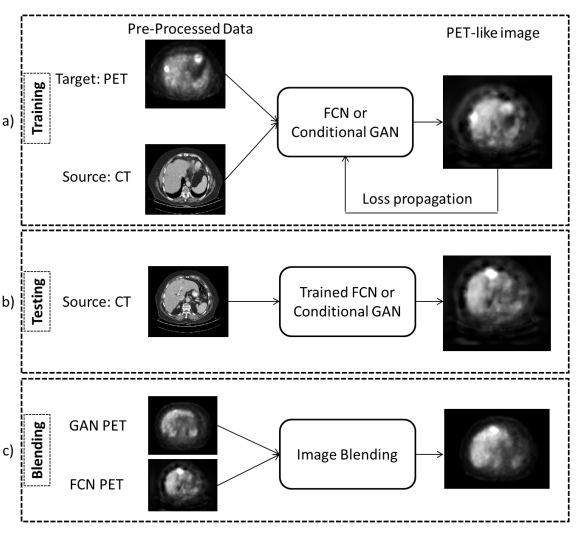
\includegraphics[scale=0.7]{ann10_sys.png} \\
        \caption{\scriptsize{Предложенная система по созданию виртуальных ПЭТ-изображений.}}
    \end{center}
    
\end{minipage}
\\
\\
\\
Так как GAN обучается созданию реалистичных ПЭТ-изображений, результат его 
работы был намного ближе к реальным ПЭТ-изображениям, чем у FCN, который воспроизвел 
размытые изображения. Однако, FCN показал лучший результат на злокачественных
образованиях, чем GAN. Авторы использовали достоинства каждого метода, чтобы создать 
смешанное изображение, которое соединяет в себе реалистичность от GAN и более точный ответ 
о злокачественности от FCN. Сперва создается маска из выходного изображения FCN, которое 
содержит регионы с повышенным SUV (>2.5). По этой маске берется часть изображения из FCN, а 
остальная достраивается из изображения от GAN.

\subsection*{Данные}
Датасет включает в себя ПЭТ изображения печени (с опухолями и без) и соответствующие им
КТ изображения из Медицинского центр имени Хаима Шибы  (Израиль).
\subsection*{Результаты}
Сгенерированные ПЭТ-изображения были визуаьлно оценены радиологом и сравнены с реальными ПЭТ-изображениями
для распознавания опухолей печени. Распознанный регион считается опухолью, если он имеет 
значени \(SUV_{max}>2.5\).  Для оценки были вычислены значения TPR и FPR.
Система успешно распознала 24 из 26 опухолей (TPR 92.3\%), c только 
двумя ложноположительными ответами среди всех 8 сканов (FPR 0.25).
\\
\\
\\
\begin{minipage}{1.0\linewidth}
    \begin{center}
        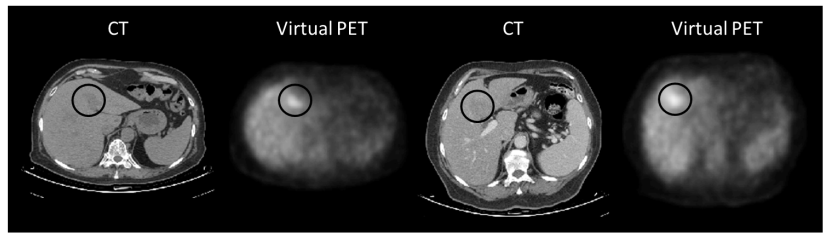
\includegraphics[scale=0.5]{ann10_res2.png} \\
        \caption{\scriptsize{Ложноположительные результаты выделены черным кругом.}}
    \end{center}
    
\end{minipage}
\subsection*{Заключение}
Была разработана система создания виртуальных ПЭТ-изображений 
по КТ изображениям с использованием FCN и GAN, которая показала 
сравнительно хорошие результаты. Работа интересная, однако, сложно представить 
ее использование в реальной жизни и степень востребованности и доверия к методу.